%%%%%%%%%%%%%%%%%%%%%%%%%%%%%%%%%%%%%%%%%%%%%%%%%%%%%%%%%%%%%%%%%%%%%%%
%%%%%%%%%%%%%%%%%%%%%%%%%%%%%%%%%%%%%%%%%%%%%%%%%%%%%%%%%%%%%%%%%%%%%%% 
%%%%%%%%%%%       								 Preamble				         	                                                        %%%%%%%%%% 
%%%%%%%%%%%%%%%%%%%%%%%%%%%%%%%%%%%%%%%%%%%%%%%%%%%%%%%%%%%%%%%%%%%%%%% 
%%%%%%%%%%%%%%%%%%%%%%%%%%%%%%%%%%%%%%%%%%%%%%%%%%%%%%%%%%%%%%%%%%%%%%% 
\documentclass[10pt]{beamer}
\usepackage{setspace}
\usepackage{color}
\usepackage{amsmath,lmodern}
\usepackage{hyperref}
\usepackage{graphicx}
\usepackage{multirow}
\usepackage{tikz}
\usetikzlibrary{fit,shapes.misc}
\usepackage{pdflscape}
\usepackage{amsmath}
\usepackage{lscape}
\usepackage{multirow}
\usepackage{enumerate}
\usepackage{epstopdf}
\usepackage{pdfpages}
\usepackage{appendixnumberbeamer}
\usepackage{color,soul}
\usepackage{grffile}
\usepackage{float}
\usepackage{relsize}
\usepackage{tcolorbox}
\newcounter{nodemarkers}
\usepackage{tikz}
\newcommand{\toplinesmall}{%
  \tikz[remember picture,overlay] {%
    \draw[blue,thick] ([yshift=-1cm, xshift=.9cm]current page.north west)
             -- ([yshift=-1cm,xshift=3.6cm]current page.north west);}}
             
\newcommand{\toplinemedium}{%
  \tikz[remember picture,overlay] {%
    \draw[blue,thick] ([yshift=-1cm, xshift=.9cm]current page.north west)
             -- ([yshift=-1cm,xshift=6.2cm]current page.north west);}}
 
 \newcommand{\toplinelarge}{%
  \tikz[remember picture,overlay] {%
    \draw[blue,thick] ([yshift=-1cm, xshift=.9cm]current page.north west)
             -- ([yshift=-1cm,xshift=8.9cm]current page.north west);}}           
             
 \newcommand{\toplinexlarge}{%
  \tikz[remember picture,overlay] {%
    \draw[blue,thick] ([yshift=-1cm, xshift=.9cm]current page.north west)
             -- ([yshift=-1cm,xshift=12cm]current page.north west);}}                       
             
\setbeamertemplate{footline}
{
  \leavevmode%
  \hbox{%
  \begin{beamercolorbox}[wd=.333333\paperwidth,ht=2.25ex,dp=1ex,center]{author in head/foot}%
    \usebeamerfont{author in head/foot}{\textcolor{blue}{ECON311}}
  \end{beamercolorbox}%
  \begin{beamercolorbox}[wd=.333333\paperwidth,ht=2.25ex,dp=1ex,center]{title in head/foot}%
    \usebeamerfont{title in head/foot}{\textcolor{blue}{Winter 2026}}
  \end{beamercolorbox}%
  \begin{beamercolorbox}[wd=.333333\paperwidth,ht=2.25ex,dp=1ex,right]{date in head/foot}%
    \usebeamerfont{date in head/foot}{\textcolor{blue}{Lecture 2 \: \: \: \: \: \: \: }
    \insertframenumber{} / \inserttotalframenumber\hspace*{2ex}} 
  \end{beamercolorbox}}%
  \vskip0pt%
}
\newtheorem{proposition}[theorem]{Proposition}

\newcommand\marktopleft[1]{%
    \tikz[overlay,remember picture] 
        \node (marker-#1-a) at (-0.2,1.2ex) {};%
}
\newcommand\markbottomright[1]{%
    \tikz[overlay,remember picture] 
        \node (marker-#1-b) at (0.16,-1ex) {};%
    \tikz[overlay,remember picture,thick,inner sep=4pt]
        \node[draw,rectangle,rounded corners, blue, fit=(marker-#1-a.center) (marker-#1-b.center)] {};%
}

\setbeamertemplate{caption}{\raggedright\insertcaption\par}
\setbeamertemplate{itemize items}[ball]
\setbeamertemplate{itemize subitem}[triangle]
\setbeamertemplate{itemize subsubitem}[triangle]
\tcbset{colframe=white,colback=white,nobeforeafter}
\beamertemplatenavigationsymbolsempty
\addtobeamertemplate{frametitle}{\vspace*{0.19cm}}{\vspace*{0cm}}


%%%%%%%%%%%%%%%%%%%%%%%%%%%%%%%%%%%%%%%%%%%%%%%%%%%%%%%%%%%%%%%%%%%%%%%
%%%%%%%%%%%%%%%%%%%%%%%%%%%%%%%%%%%%%%%%%%%%%%%%%%%%%%%%%%%%%%%%%%%%%%% 
%%%%%%%%%  									    Define Title									                                       %%%%%%%%%
%%%%%%%%%%%%%%%%%%%%%%%%%%%%%%%%%%%%%%%%%%%%%%%%%%%%%%%%%%%%%%%%%%%%%%%
%%%%%%%%%%%%%%%%%%%%%%%%%%%%%%%%%%%%%%%%%%%%%%%%%%%%%%%%%%%%%%%%%%%%%%% 
\title{ECON 311} 
\author{Lecture 2: Measuring the Aggregate Economy}
\date{}
\AtBeginSection[]
{
 \begin{frame}<beamer>
 \tableofcontents[currentsection]
 \end{frame}
}
%%%%%%%%%%%%%%%%%%%%%%%%%%%%%%%%%%%%%%%%%%%%%%%%%%%%%%%%%%%%%%%%%%%%%%%
%%%%%%%%%%%%%%%%%%%%%%%%%%%%%%%%%%%%%%%%%%%%%%%%%%%%%%%%%%%%%%%%%%%%%%% 
%%%%%%%% 						     				Document								                                                %%%%%%%%
%%%%%%%%%%%%%%%%%%%%%%%%%%%%%%%%%%%%%%%%%%%%%%%%%%%%%%%%%%%%%%%%%%%%%%%
%%%%%%%%%%%%%%%%%%%%%%%%%%%%%%%%%%%%%%%%%%%%%%%%%%%%%%%%%%%%%%%%%%%%%%% 
\begin{document}
\setbeamercovered{transparent}

\begin{frame}
\maketitle
\end{frame}

%%%%%%%%%%%%%%%%%%%%%%%%%%%%%%%%%%%%%%%%%%%%%%%%%%%%%%%%%%%%%%%%%%%%%%%
%%%%%%%%%%%%%%%%%%%%%%%%%%%%%%%%%%%%%%%%%%%%%%%%%%%%%%%%%%%%%%%%%%%%%%% 
%%%%%%%% 						     				Introduction	             		                                		  %%%%%%%%
%%%%%%%%%%%%%%%%%%%%%%%%%%%%%%%%%%%%%%%%%%%%%%%%%%%%%%%%%%%%%%%%%%%%%%%
%%%%%%%%%%%%%%%%%%%%%%%%%%%%%%%%%%%%%%%%%%%%%%%%%%%%%%%%%%%%%%%%%%%%%%% 

\section{Measuring the Macroeconomy}

\begin{frame}
\frametitle{\: \: \: Measuring the Macroeconomy}
\toplinelarge
To study the macroeconomy, we need a \textbf{statistic} that summarizes the state of overall economic activity in a country.
\begin{itemize}
\vspace{.11in}
\item The most important measure of the state of the economy is \textbf{GDP:}
\vspace{.18in}
\begin{center}
\textit{GDP is the market value of all final goods and services produced  within a country in a given period of time}
\end{center}
\end{itemize}
\end{frame}

\begin{frame}
\frametitle{\: \: \: GDP per capita and well-being}
\toplinexlarge
\begin{figure}
\centering
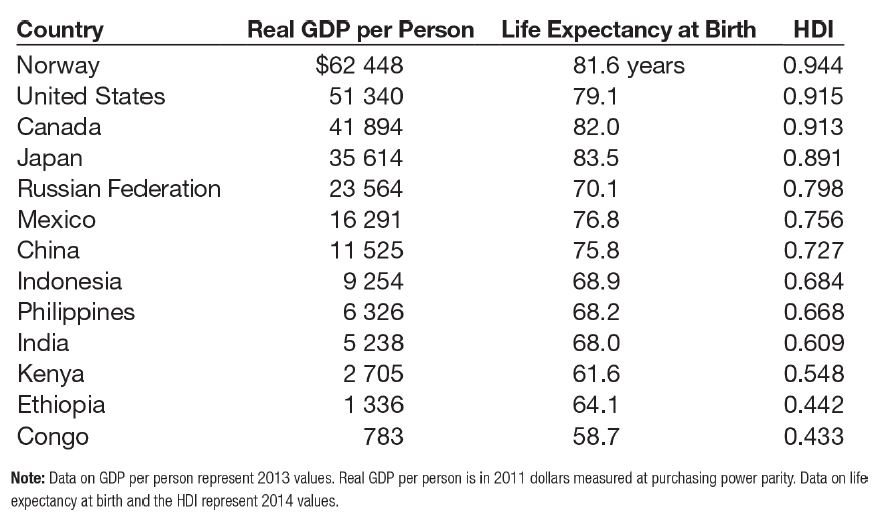
\includegraphics[scale=.45]{GDP_welfare}
\caption{Source: Principles of Macroeconomics, 7ce}
\end{figure}
\end{frame}

\begin{frame}
\frametitle{\: \: \: GDP per capita and well-being}
\toplinexlarge
\begin{figure}
\centering
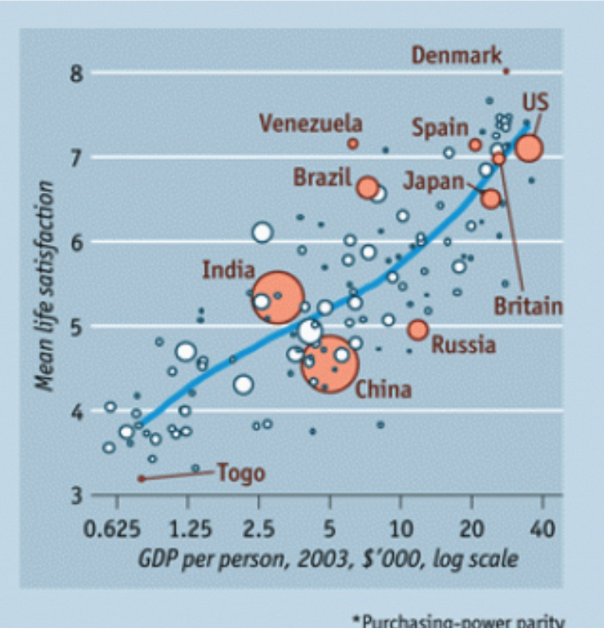
\includegraphics[scale=.5]{GDP_satisfaction}
\caption{GDP and Life Satisfaction}
\end{figure}
\end{frame}

\begin{frame}
\frametitle{\: \: \: GDP per capita and well-being}
\toplinexlarge
\begin{itemize}
\item GDP per capita is only an imperfect measure of well-being because it does not affect several factors that affect living standards such as:
\begin{itemize}
\vspace{.11in}
\item the value of leisure
\vspace{.11in}
\item the value of a clean environment
\vspace{.11in}
\item the value of any non-market activity
\end{itemize}
\end{itemize}
\end{frame}

%%%%%%%%%%%%%%%%%%%%%%%%%%%%%%%%%%%%%%%%%%%%%%%%%%%%%%%%%%%%%%%%%%%%%%%
%%%%%%%%%%%%%%%%%%%%%%%%%%%%%%%%%%%%%%%%%%%%%%%%%%%%%%%%%%%%%%%%%%%%%%% 
%%%%%%%% 						     				 National Accountings	             		                                		  %%%%%%%%
%%%%%%%%%%%%%%%%%%%%%%%%%%%%%%%%%%%%%%%%%%%%%%%%%%%%%%%%%%%%%%%%%%%%%%%
%%%%%%%%%%%%%%%%%%%%%%%%%%%%%%%%%%%%%%%%%%%%%%%%%%%%%%%%%%%%%%%%%%%%%%% 
\section{National Accounting}

\begin{frame}
\frametitle{\: \: \: Measuring Value of Production}
\toplinexlarge
There are three equivalent approaches to measuring the value of production of final goods and services:
\begin{enumerate}
\vspace{.11in}
\item Expenditure approach
\vspace{.11in}
\item Income approach
\vspace{.11in}
\item Production approach
\end{enumerate}
\end{frame}

\begin{frame}
\frametitle{\: \: \: Expenditure Approach}
\toplinemedium
\begin{eqnarray*}
Y=C+I+G+NX
\end{eqnarray*}
\begin{itemize}
\item Y=GDP (in dollars)
\item C=consumption
\item I=investment
\item G=government purchases
\item NX=exports-imports
\end{itemize}
\end{frame}

\begin{frame}
\frametitle{\: \: \: Expenditure Approach}
\toplinemedium
\begin{figure}
\centering
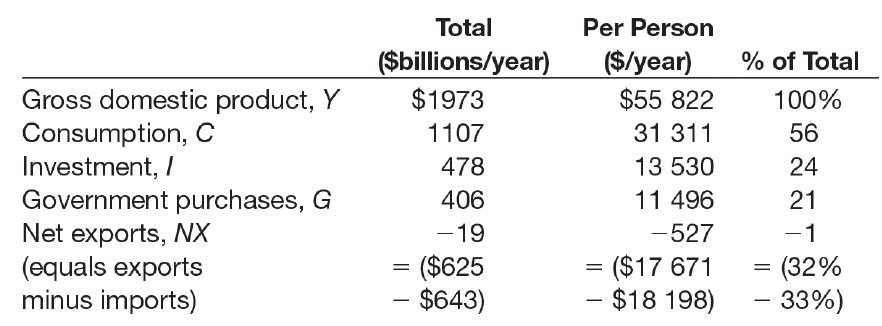
\includegraphics[scale=.43]{expenditure_approach_can}
\caption{GDP in Canada 2014, expenditure approach}
\end{figure}
\end{frame}

\begin{frame}
\frametitle{\: \: \: Expenditure Approach}
\toplinemedium
\begin{figure}
\centering
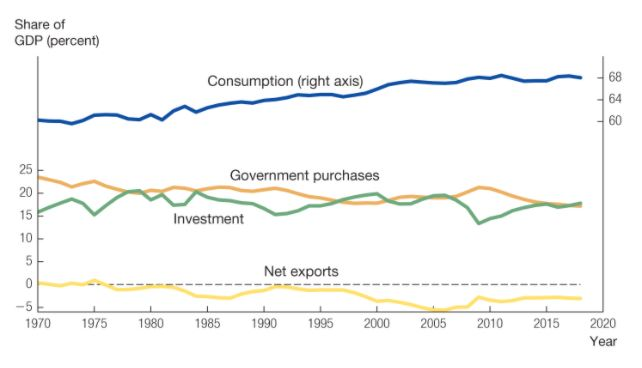
\includegraphics[scale=.65]{share_GDP_expenditure_approach}
\caption{Notes: Expenditure Shares of US GDP. Source: Macroeconomics, Jones}
\end{figure}
\end{frame}


\begin{frame}
\frametitle{\: \: \: Income Approach}
\toplinemedium
\begin{figure}
\centering
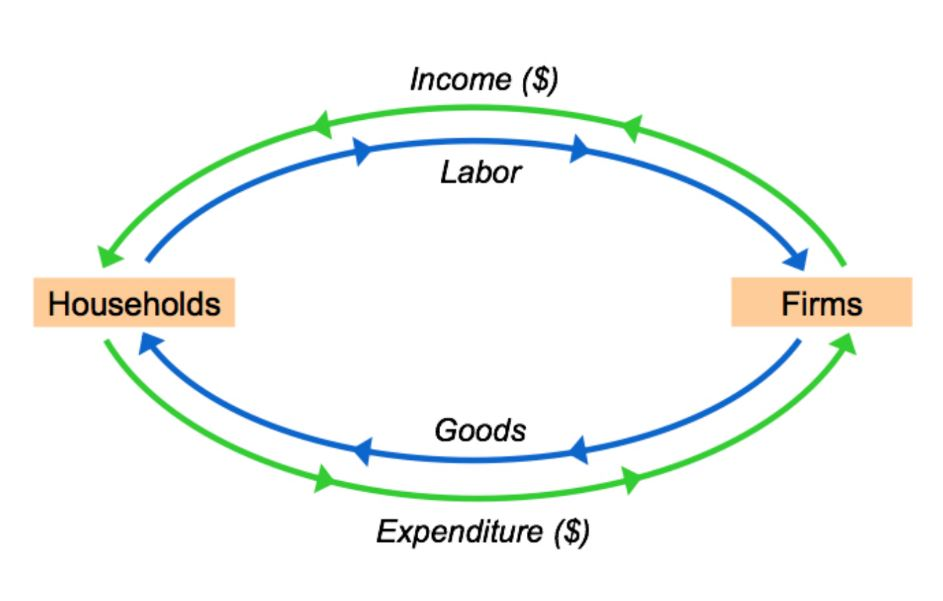
\includegraphics[scale=.35]{circular_flow}
\end{figure}
\end{frame}

\begin{frame}
\frametitle{\: \: \: Income Approach}
\toplinemedium
\begin{figure}
\centering
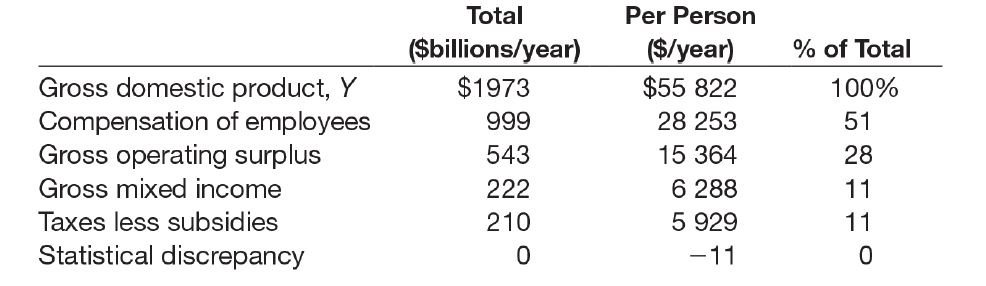
\includegraphics[scale=.43]{income_approach_can}
\caption{GDP in Canada 2014, income approach}
\end{figure}
\end{frame}

\begin{frame}
\frametitle{\: \: \: Income Approach}
\toplinemedium
\begin{figure}
\centering
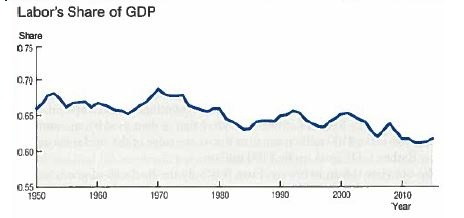
\includegraphics[scale=.65]{labour_share}
\caption{Source: Macroeconomics, Jones}
\end{figure}
\end{frame}

\begin{frame}
\frametitle{\: \: \: Production Approach}
\toplinemedium
\begin{itemize}
\item The production approach is based on counting the \textit{value-added} at each stage of production
\begin{itemize}
\vspace{.11in}
\item E.g. in a car assembly line, this approach only accounts for worker's wages but not for the value of intermediate inputs (i.e. the different parts of the car)
\end{itemize}
\vspace{.11in}
\item In practice, it is very hard to obtain reliable \textit{value-added} data for all sectors, ...
\begin{itemize}
\vspace{.11in}
\item so the production approach is rarely used.
\end{itemize}
\end{itemize}
\end{frame}

%%%%%%%%%%%%%%%%%%%%%%%%%%%%%%%%%%%%%%%%%%%%%%%%%%%%%%%%%%%%%%%%%%%%%%%
%%%%%%%%%%%%%%%%%%%%%%%%%%%%%%%%%%%%%%%%%%%%%%%%%%%%%%%%%%%%%%%%%%%%%%% 
%%%%%%%% 			                                      	Measuring Changes Across Time		   	                                                       %%%%%%%%
%%%%%%%%%%%%%%%%%%%%%%%%%%%%%%%%%%%%%%%%%%%%%%%%%%%%%%%%%%%%%%%%%%%%%%%
%%%%%%%%%%%%%%%%%%%%%%%%%%%%%%%%%%%%%%%%%%%%%%%%%%%%%%%%%%%%%%%%%%%%%%% 
\section{Measuring Changes Across Time}

\begin{frame}
\frametitle{\: \: \: GDP across time}
\toplinemedium
We call the sum of the value of production at a particular time ($t$), nominal GDP:
\begin{eqnarray*}
NGDP_t=\underset{i=1}{\overset{N}{\mathlarger{\sum}}}p_{i,t} \cdot q_{i,t} &, & i=1, ..., N,  (e.g \: \: \: t=2018)
\end{eqnarray*}
\begin{itemize}
\item $\Delta NGDP$ across time happens because:
\begin{enumerate}
\vspace{.11in}
\item $\Delta p_i$
\vspace{.11in}
\item $\Delta q_i$
\end{enumerate}
\vspace{.11in}
\item To measure real changes in the economy, we need to separate $2$ from $1$  
\end{itemize}
\end{frame}

\begin{frame}
\frametitle{\: \: \: Quantity Indexes}
\toplinemedium
Suppose we want to measure real changes between 2018 and 2019, there are two widely used quantity indexes
\begin{enumerate}
\item Laspeyres:
\begin{eqnarray*}
RGDP_{2018}^{2018 \$}= \underset{i=1}{\overset{N}{\mathlarger{\sum}}}p_{i,2018} \cdot q_{i,2018} & RGDP_{2019}^{2018 \$}= \underset{i=1}{\overset{N}{\mathlarger{\sum}}}p_{i,2018} \cdot q_{i,2019} 
\end{eqnarray*}
\begin{eqnarray*}
\% \Delta RGDP_{L}=\frac{ RGDP_{2019}^{2018 \$}-RGDP_{2018}^{2018 \$}}{RGDP_{2018}^{2018 \$}}*100
\end{eqnarray*}
\item Paasche: 
\begin{eqnarray*}
RGDP_{2018}^{2019 \$}= \underset{i=1}{\overset{N}{\mathlarger{\sum}}}p_{i,2019} \cdot q_{i,2018} & RGDP_{2019}^{2019 \$}= \underset{i=1}{\overset{N}{\mathlarger{\sum}}}p_{i,2019} \cdot q_{i,2019}  
\end{eqnarray*}
\begin{eqnarray*}
\% \Delta RGDP_{P}=\frac{ RGDP_{2019}^{2019 \$}-RGDP_{2018}^{2019 \$}}{RGDP_{2018}^{2019 \$}}*100
\end{eqnarray*}
\end{enumerate}
\end{frame}
 
\begin{frame}
\frametitle{\: \: \: Quantity Indexes}
\toplinemedium
\begin{itemize}
\item The only time $\% \Delta RGDP_{L}=\% \Delta RGDP_{P}$ is when either all prices or all quantities change proportionaly, or both.
\vspace{.11in}
\item To partially correct for this, a weighted average between the two years, called the Fisher index is implemented:
\begin{eqnarray*}
\% \Delta RGDP_{F}= \frac{\% \Delta RGDP_{L}+\% \Delta RGDP_{P}}{2}
\end{eqnarray*}
\end{itemize}
\end{frame}

\begin{frame}
\frametitle{\: \: \: Example-- Calculating Chained Prices RGDP}
\toplinexlarge
\only<1>{
\begin{table}[!t]
\begin{minipage}[h]{1\textwidth}
\centering
\resizebox{10.6cm}{!}{%
\begin{tabular}{lccccc}
\hline
Year           & $P_{apple}$  &   $Q_{apple}$  & $P_{computer}$  &   $Q_{computer}$ &  NGDP \\
\hline
2018          &1                       & 500                   &900                    &  5                            & $\$5000$ \\
2019	    &2                       & 600                  &1000                   &  5                            &$\$6200$ \\
2020         &3                       & 700                    &1000                   &  6                            &$\$8100$ \\
\hline
\hline
\end{tabular}}
\end{minipage}
\end{table}}
\only<2>{
\begin{table}[!t]
\begin{minipage}[h]{1\textwidth}
\centering
\resizebox{10.6cm}{!}{%
\begin{tabular}{lccccc}
\hline
Year           & $P_{apple}$  &   $Q_{apple}$  & $P_{computer}$  &   $Q_{computer}$ & $\% \Delta RGDP_{L}$  \\
\hline
2018          &1                       & 500                   &900                    &  5                            &                 \\
2019	    &2                       & 600                   &1000                   &  5                            & $2\%$       \\
2020         &3                       & 700                    &1000                   &  6                            & $19.35\%$ \\
\hline
\hline
\end{tabular}}
\end{minipage}
\end{table}}
\only<3>{
\begin{table}[!t]
\begin{minipage}[h]{1\textwidth}
\centering
\resizebox{10.6cm}{!}{%
\begin{tabular}{lccccc}
\hline
Year           & $P_{apple}$  &   $Q_{apple}$  & $P_{computer}$  &   $Q_{computer}$ & $RGDP_{L}$ Chained Prices   \\
                 &                       &                         &                             &                              & benchmarked to 2020        \\
\hline
2018          &1                       & 500                   &900                    &  5                            &   $\$6650.9$                       \\
2019	    &2                       & 600                   &1000                   &  5                            &   $\$6783.9$                       \\
2020         &3                       & 700                    &1000                   &  6                            &  $\$8100$                          \\
\hline
\hline
\end{tabular}}
\end{minipage}
\end{table}}
\only<4>{
\begin{table}[!t]
\begin{minipage}[h]{1\textwidth}
\centering
\resizebox{10.6cm}{!}{%
\begin{tabular}{lccccc}
\hline
Year           & $P_{apple}$  &   $Q_{apple}$  & $P_{computer}$  &   $Q_{computer}$ & $\% \Delta RGDP_{P}$  \\
\hline
2018          &1                       & 500                   &900                    &  5                            &                 \\
2019	    &2                       & 600                   &1000                   &  5                            & $3.3\%$       \\
2020         &3                       & 700                    &1000                   &  6                            & $19.12\%$ \\
\hline
\hline
\end{tabular}}
\end{minipage}
\end{table}}
\only<5>{
\begin{table}[!t]
\begin{minipage}[h]{1\textwidth}
\centering
\resizebox{10.6cm}{!}{%
\begin{tabular}{lccccc}
\hline
Year           & $P_{apple}$  &   $Q_{apple}$  & $P_{computer}$  &   $Q_{computer}$ & $RGDP_{P}$ Chained Prices   \\
                 &                       &                         &                             &                              & benchmarked to 2020        \\
\hline
2018          &1                       & 500                   &900                    &  5                            &   $\$6583.7$                       \\
2019	    &2                       & 600                   &1000                   &  5                            &   $\$6801$                       \\
2020         &3                       & 700                    &1000                   &  6                            &  $\$8100$                          \\
\hline
\hline
\end{tabular}}
\end{minipage}
\end{table}}
\only<6>{
\begin{table}[!t]
\begin{minipage}[h]{1\textwidth}
\centering
\resizebox{10.6cm}{!}{%
\begin{tabular}{lccccc}
\hline
Year           & $P_{apple}$  &   $Q_{apple}$  & $P_{computer}$  &   $Q_{computer}$ & $\% \Delta RGDP_{F}$  \\
\hline
2018          &1                       & 500                   &900                    &  5                            &                 \\
2019	    &2                       & 600                   &1000                   &  5                            & $2.65\%$       \\
2020         &3                       & 700                    &1000                   &  6                            & $19.24\%$ \\
\hline
\hline
\end{tabular}}
\end{minipage}
\end{table}}
\only<7>{
\begin{table}[!t]
\begin{minipage}[h]{1\textwidth}
\centering
\resizebox{10.6cm}{!}{%
\begin{tabular}{lccccc}
\hline
Year           & $P_{apple}$  &   $Q_{apple}$  & $P_{computer}$  &   $Q_{computer}$ & RGDP Chained Weighted Prices   \\
                 &                       &                         &                             &                              & benchmarked to 2020        \\
\hline
2018          &1                       & 500                   &900                    &  5                            &   $\$6616.7$                       \\
2019	    &2                       & 600                   &1000                   &  5                            &   $\$6795.3$                       \\
2020         &3                       & 700                    &1000                   &  6                            &  $\$8100$                          \\
\hline
\hline
\end{tabular}}
\end{minipage}
\end{table}}
\end{frame}

\begin{frame}
\frametitle{\: \: \: Price Indexes and Inflation}
\toplinelarge
\begin{itemize}
\item To calculate price changes across time, we use price indexes:
\begin{eqnarray*}
GDP^{deflator}_t=\frac{NGDP_t}{RGDP_t}
\end{eqnarray*}
\begin{eqnarray*}
Inflation_t=\frac{GDP^{deflator}_t-GDP^{deflator}_{t-1}}{GDP^{deflator}_{t-1}}
\end{eqnarray*}
\end{itemize}
\end{frame}

\begin{frame}
\frametitle{\: \: \: Example-- Price Indexes and Inflation}
\toplinexlarge
\begin{table}[!t]
\begin{minipage}[h]{1\textwidth}
\centering
\resizebox{10.6cm}{!}{%
\begin{tabular}{lcccc}
\hline
Year           &NGDP & RGDP Chained Weighted Prices  &$GDP^{deflator}$ & Inflation Rate  \\
                 &            & benchmarked to 2020                  &                           &                \\
\hline
2018          & $\$5000$   &   $\$6616.7$                          &           0.756               &                    \\
2019	    &   $\$6200$     &   $\$6795.3$                      &           0.912                &   $20.63\%$                 \\
2020         &     $\$8100$   &  $\$8100$                          &             1               &      $9.75\%$               \\
\hline
\hline
\end{tabular}}
\end{minipage}
\end{table}
\end{frame}

\begin{frame}
\frametitle{\: \: \: GDP Across Time-- Conclusion}
\toplinexlarge
\begin{itemize}
\item We use Quantity and Price Indexes to separate the effect of changes in real quantities from changes in prices.
\vspace{.11in} 
\item An alternative and simpler way of calculating quantity and price indexes is to use constant prices for a given year
\begin{itemize}
\vspace{.11in}
\item Introduce problems when used over long periods in cases where
\begin{itemize}
\vspace{.11in}
\item relative prices of goods changes because of changes in their relative quality (e.g. computers) 
\end{itemize}
\vspace{.11in}
\item Chain Weighting solves this issue by both...
\begin{itemize}
\vspace{.11in}
\item considering short time periods (chain)
\vspace{.11in}
\item combining information from both current and future prices (weight)
\end{itemize}
\end{itemize}
\end{itemize}
\end{frame}

%%%%%%%%%%%%%%%%%%%%%%%%%%%%%%%%%%%%%%%%%%%%%%%%%%%%%%%%%%%%%%%%%%%%%%%
%%%%%%%%%%%%%%%%%%%%%%%%%%%%%%%%%%%%%%%%%%%%%%%%%%%%%%%%%%%%%%%%%%%%%%% 
%%%%%%%% 			                       Measuring Differences Across Countries		  %%%%%%%%
%%%%%%%%%%%%%%%%%%%%%%%%%%%%%%%%%%%%%%%%%%%%%%%%%%%%%%%%%%%%%%%%%%%%%%%
%%%%%%%%%%%%%%%%%%%%%%%%%%%%%%%%%%%%%%%%%%%%%%%%%%%%%%%%%%%%%%%%%%%%%%% 
\section{Measuring Differences Across Countries}

\begin{frame}
\frametitle{\: \: \: Differences in Economic Activity Across Countries}
\toplinexlarge
\begin{itemize}
\item We could compare NGDP using a common currency (e.g. transform Canadian NGDP in US Dollars):
\begin{eqnarray*}
NGDP_{CAN}^{USD}=\frac{1}{e_{CAD/USD}} NGDP_{CAN}^{CAD}
\end{eqnarray*}
\begin{itemize}
\item $e_{CAD/USD}$ does not perfectly reflect differences in prices across countries (e.g. differences in production costs)...
\begin{itemize}
\vspace{.11in}
\item so comparing $NGDP_{CAN}^{USD}$ with $NGDP_{US}^{USD}$ has the same problem as comparing $NGDP$ across time
\end{itemize} 
\end{itemize}
\vspace{.11in}
\item To control for price differences, we use (PPP) 
\begin{eqnarray*}
RGDP_{CAN}^{USD}=\frac{P_{US}}{P^{USD}_{CAN}}NGDP_{CAN}^{USD} 
\end{eqnarray*}
\item In practice, we usually use Chain-Weighting to facilitate comparison across time
\end{itemize}
\end{frame}

\begin{frame}
\frametitle{\: \: \: RGDP Across Countries}
\toplinelarge
\begin{table}[!t]
\begin{minipage}[h]{1\textwidth}
\centering
\resizebox{11cm}{!}{%
\begin{tabular}{l|c|c|c}
\hline
                                                 & Canada 				       &   United States 		      &Mexico     \\
\hline
GDP Growth                           &$1.7\% $   				   &$1.7\% $				     &$1.4\% $\\		
GDP per head                          &$\$57,190$(PPP:$\$67,090$)&$\$86,190$(PPP:$\$86,190$) &$\$14,290$(PPP:$\$27,060$) \\
Inflation                                   &$2.2\% $  				   &$3.0\% $				     &$4.0\% $  \\
Budget Balance ($\%$ GDP)    &-1.0						   &-6.9						     &-4.0      \\
Population                               &40.1M      				   &347.3M					     &131.9M   \\ 
\hline
\end{tabular}}
\end{minipage}
\end{table}
\end{frame}


\section{Introduction to Long-Run Growth}

\begin{frame}
\frametitle{\: \: \: Introduction to Growth}
\toplinelarge
\begin{itemize}
\item Standards of living in industrialized countries have greatly increased over the past few centuries.
\begin{itemize}
\vspace{.11in}
\item E.g. Averages incomes today in North America and Western Europe are between 50 and 300 times larger than two centuries ago.
\end{itemize}
\vspace{.11in}
\item This increase in standards of living has been a very recent phenomena in human history.
\begin{itemize}
\vspace{.11in}
\item For most of their history (before the Industrial Revolution), humans lived barely above subsistence levels.
\end{itemize}
\vspace{.11in}
\item Economic growth has been very uneven across time.
\begin{itemize}
\vspace{.11in}
\item E.g. the productivity growth slowdown of 1990's
\end{itemize}
\vspace{.11in}
\item Economic growth has been very uneven across countries. 
\begin{itemize}
\vspace{.11in}
\item E.g. growth miracles (Japan, South Korea, Singapore), growth disasters (Argentina, Sub-Saharan countries)
\end{itemize}
\end{itemize}
\end{frame}

\begin{frame}
\frametitle{\: \: \: Economic Growth Over the Very Long Run}
\toplinexlarge
\begin{figure}
\centering
\includegraphics[scale=.63]{econ_growth.png}
\caption{Source: Macroeconomics, Jones}
\end{figure}
\end{frame}

\begin{frame}
\frametitle{\: \: \: Economic Growth Over Time}
\toplinelarge
\begin{figure}
\centering
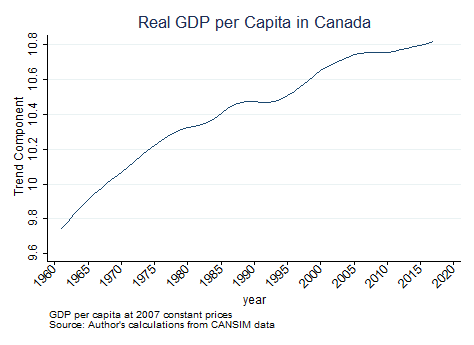
\includegraphics[scale=.56]{RGDP_trend}
\end{figure}
\end{frame}

\begin{frame}
\frametitle{\: \: \: Defining Economic Growth}
\toplinelarge
\begin{itemize}
\item Let $g$ be a constant growth rate over a period of time, then ...
\begin{eqnarray*}
y_{t+T}=y_{t}(1+g)^{T} 
\end{eqnarray*}
\item Important properties of growth rates:
\begin{enumerate}
\vspace{.11in}
\item (Rule of 70) Let $y_{t+T}=2y_t$ and , then
\begin{eqnarray*}
T \approx \frac{0.7}{g}
\end{eqnarray*}
\item In general, the time it takes for a series to increase by a certain ratio does not depend on the initial level.
\vspace{.11in}
\item Algebraic properties of growth rates (let the variable $i$ grow at a constant growth rate $g_i$):
\begin{eqnarray*}
\begin{array}{cl} 
z=\frac{x}{y} & \Rightarrow g_z \approx g_x-g_y \\
z=x \cdot y &\Rightarrow g_z \approx g_x+g_y \\
z=x^a \text{ (where $a$ is a constant)} & \Rightarrow g_z \approx a\cdot g_x
\end{array}
\end{eqnarray*}
\end{enumerate}
\end{itemize}
\end{frame}



\end{document}


